\chapter{Développement}

\section{Fonctionnalités du jeu}

Ce jeu est un mélange entre les jeux de types Tower Defense, et les jeux Zelda.
Le joueur a le contrôle de Link et a accès à tous les endroits du terrain de
jeu, mis à part quelques obstacles comme les murs ou comme les flaques d'eau.
En revanche, les \emph{creeps} sont restreints aux terrains de type
"Path", comme dans certains Tower Defense, et ne peuvent en aucun cas quitter le chemin, et il est
impossible de les y contraindre.\\
Il existe une condition de défaite: lorsque Zelda (destination finale des
\emph{creeps}) n'a plus de points de vie, la partie est perdue.
La condition de victoire est d'éliminer tous les \emph{creeps} que les Spawns
prévoient d'envoyer à l'assaut de la princesse.
Link n'est lui même pas invulnérable, il possède un certain nombre de points
de vie aussi. S'il percute un mur (en se faisant éjecter dans un mur au
contact d'un \emph{creep}), il ne perdra pas de points de vie, mais il sera
renvoyé à son point d'apparition initiale.
Si ses points de vie atteignent zéro, il sera également renvoyé à son point
d'origine, et son compteur de vie sera initialisé à trois.\\
Link possède deux équipements: son épée, et son bouclier.\\
Lorsque Link équipe son épée, il peut frapper les \emph{creeps}, ainsi les
repoussant, et leur infligeant des dégâts.\\
Lorsque Link équipe son bouclier, il peut repousser les \emph{creeps}, de la
même manière qu'avec l'épée, mais ce sans infliger de dégâts.\\


\section{Modifications du framework}

Afin de pouvoir définir des tailles de sprite différentes et rectangulaires,
nous avons créé notre propre classe OctolinkSpriteManager. Cela nous a également
permi de créer des bounding box avec des tailles personnalisées et de bien les
aligner par rapport aux sprites. Nous avons été obligé de dupliquer la classe
IntersectTools du framework existant pour gérer les collisions correctement avec
nos bounding box personnalisées.

\begin{figure}[ht!]
  \center
  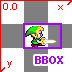
\includegraphics{resources/bbox.png}
  \caption{Link sprite bounding box}
  \label{fig:Link sprite bounding box}
\end{figure}

De plus, pour rajouter une barre de vie pour Zelda et implémenter les fonctions
\emph{pause} et \emph{resume}, nous avons été contraints de dupliquer les
classes GameDefaultImpl et GameLevelDefaultImpl.


\section{Architecture du jeu}

\begin{figure}[ht!]
  \center
  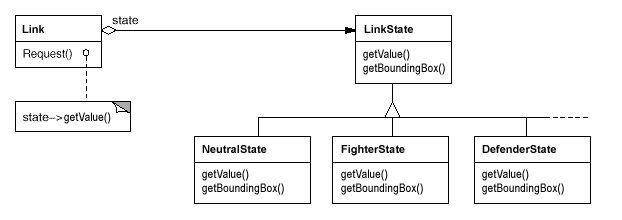
\includegraphics[width=16cm,keepaspectratio]{resources/state_pattern.png}
  \caption{State pattern}
  \label{fig:State pattern}
\end{figure}


\section{Problèmes rencontrés}
La modification des bounding box engendrée par l'utilisation de sprites de
tailles différents a été complexe car il a fallu intégrer les modifications au
système de gestion des collisions.
L'implémentation des fonctions \emph{pause} et \emph{resume} s'est avérée assez
délicate à cause de la gestion des Threads avec les méthodes \emph{wait()} et
\emph{notify()} en étant \emph{synchronized}.
